\documentclass[../main.tex]{subfiles}

\begin{document}
\section{Gondola Arm Deflection}
To ensure that the gondola will not fall off of the keel during operation, a deflection calculation is computed on the gondola arm. The maximum deflection of the gondola arm is modelled as shown below:

\begin{figure}[H]
	\centering
	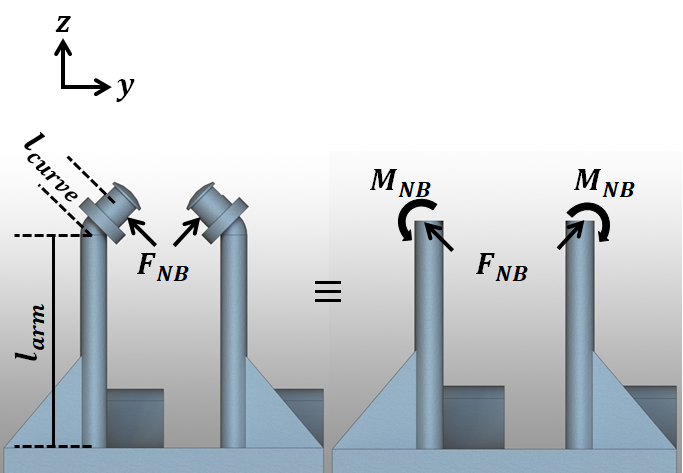
\includegraphics[width=.8\linewidth]{img/gondola/armDeflection.PNG}
	\caption{Model Used to Compute the Deflection of the Gondola Arms}
	\label{fig:deflection}
\end{figure}

For the sake of simplicity, the curved section at the very top is ignored and the force is translated from the curved section to the straight section using a force-moment couple. The moment $M_{NB}$ is computed as $M_{NB}=F_{NB}l_{curve}$. Furthermore, the rib seen in Figure \ref{fig:deflection} is ignored. The deflection criteria will be computed without the rib, and the rib will be added as an extra preventative measure, to ensure the member is rigid enough.\\

The deflection will be calculated using simple beam equations. The force $F_{NB}$ is resolved into $y$ and $z$ components. The deflection is then computed in three separate parts, as shown below:

\begin{align}
	\delta _{Gondola Arm} = \delta _{axial} + \delta _{bending force} + \delta _{bending moment} \\ \label{armDeflection}
	\delta _{Gondola Arm}  = \left(\dfrac{F_{NB_{z}}l_{arm}}{AE}\right)\hat{k} + \left(\dfrac{F_{NB_{y}}l_{arm}^3}{3EI}  + \dfrac{M_{NB}l_{arm}^2}{2EI} \right) \hat{j}
\end{align}

The faliure possibility here would be for the arm to deflect enough that the gondola falls of the keel. This occurs when the total deflection $\delta$ is larger than $0.5cm$, which is half of the width of the keel face. Therefore it is required that the result of Equation \ref{armDeflection} be less than $0.5cm$.

\end{document}